\chapter[\textit{pyenv}]{\textit{pyenv} \\ Simplifier la gestion \\ des versions de Python}

\insertcitation{Sois comme l’eau : elle s’adapte à toute forme sans jamais perdre sa nature.}{Citation taoïste}
\bigskip

À mesure que l’on progresse dans la pratique du langage Python, une réalité s’impose : tous les projets ne parlent pas le même dialecte. Certains réclament une version ancienne, d’autres tirent parti des nouveautés les plus récentes. Installer plusieurs versions de Python sur une même machine peut alors devenir source de confusion, voire de conflit.

C’est ici qu’intervient \textbf{pyenv}, un outil discret mais très efficace, qui permet de jongler aisément entre les versions de Python. À la manière de l’eau qui épouse la forme du vase sans jamais perdre sa nature, \textbf{pyenv} s’adapte à chaque projet, chaque environnement, sans rien imposer au système global.

Ce chapitre nous guidera pas à pas dans la découverte et l’utilisation de \textbf{pyenv} : de son installation à sa maîtrise au quotidien. L’objectif n’est pas seulement de fournir un outil de plus, mais de proposer une nouvelle manière d’interagir avec notre environnement de développement — plus souple, plus propre, et infiniment plus adaptée.

Page \textbf{GitHub} du projet \textbf{pyenv} : \url{https://github.com/pyenv/pyenv}

\section{Installer \textit{pyenv}}
Avant d'installer \textbf{pyenv} lui-même, nous aurons besoin de quelques dépendances spécifiques à notre système d'exploitation. Ces dépendances sont principalement des utilitaires de développement écrits en \textbf{C} et sont nécessaires parce que \textbf{pyenv} installe Python en le construisant à partir des sources.

\subsection*{Les dépendances de construction}
Les dépendances de construction varient selon la plate-forme. Sur \textbf{Debian GNU/Linux} il nous faudra installer les dépendances suivantes :
\begin{lstlisting}[style=bash]
|\userprompt| sudo apt install -y make build-essential libssl-dev zlib1g-dev libbz2-dev libreadline-dev libsqlite3-dev wget curl llvm libncurses5-dev libncursesw5-dev xz-utils tk-dev libffi-dev liblzma-dev python3-openssl
\end{lstlisting}

\subsection*{Utiliser le programme d'installation de \textit{pyenv}}
Après avoir installé les dépendances, nous sommes prêts à installer \textbf{pyenv} lui-même. Il est recommandé d'utiliser le projet \textbf{pyenv-installer}\footnote{\url{https://github.com/pyenv/pyenv-installer}}.
\begin{lstlisting}[style=bash]
|\userprompt| curl https://pyenv.run |\textbar| bash
\end{lstlisting}

Ceci installera \textbf{pyenv} ainsi que quelques \textit{plugins} utiles :
\begin{description}
    \item[pyenv]: L'application \textbf{pyenv} actuelle
    \item[pyenv-virtualenv] : \textit{Plugin} pour \textbf{pyenv} et les environnements virtuels
    \item[pyenv-update] : \textit{Plugin} pour mettre à jour \textbf{pyenv}
    \item[pyenv-doctor] : \textit{Plugin} pour vérifier que \textbf{pyenv} et les dépendances sont installés
    \item[pyenv-which-ext] : \textit{Plugin} pour rechercher automatiquement les commandes système
\end{description}
\bigskip

Pour utiliser \textbf{pyenv} avec \textbf{zsh} :
\begin{lstlisting}[style=bash]
|\userprompt| echo 'export PYENV_ROOT="$HOME/.pyenv"' >> ~/.zshrc
|\userprompt| echo '[[ -d $PYENV_ROOT/bin ]] && export PATH="$PYENV_ROOT/bin:$PATH"' >> ~/.zshrc
|\userprompt| echo 'eval "$(pyenv init - zsh)"' >> ~/.zshrc 
\end{lstlisting}

Puis relancer le \textit{shell} :
\begin{lstlisting}[style=bash]
|\userprompt| exec "\$SHELL"
\end{lstlisting}

\subsection*{Désinstaller \textit{pyenv}}
Saisir la commande \verb|rm -Rf ~/.pyenv|, puis supprimer les lignes ajoutées au fichier \texttt{.zshrc}. Et enfin, relancer le \textit{shell}.

\subsection*{Mettre à jour \textit{pyenv}}
Passons par exemple de la version \textbf{2.5.7} à la dernière version en cours\footnote{Manipulation réalisée le 13.06.2025} :
\begin{lstlisting}[style=bash]
|\userprompt| cd ~/.pyenv
|\userprompt| git pull
remote: Enumerating objects: 59, done.
remote: Counting objects: 100% (59/59), done.
remote: Compressing objects: 100% (21/21), done.
remote: Total 49 (delta 33), reused 38 (delta 25), pack-reused 0 (from 0)
[...]
 14 files changed, 92 insertions(+), 12 deletions(-)
 create mode 100644 plugins/python-build/share/python-build/3.10.18
 create mode 100644 plugins/python-build/share/python-build/3.11.13
 create mode 100644 plugins/python-build/share/python-build/3.12.11
 create mode 100644 plugins/python-build/share/python-build/3.13.4
 create mode 100644 plugins/python-build/share/python-build/3.13.4t
 create mode 100644 plugins/python-build/share/python-build/3.13.5
 create mode 100644 plugins/python-build/share/python-build/3.13.5t
 delete mode 100644 plugins/python-build/share/python-build/3.14.0b1t
 rename plugins/python-build/share/python-build/{3.14.0b1 => 3.14.0b2} (59%)
 create mode 100644 plugins/python-build/share/python-build/3.14.0b2t
 create mode 100644 plugins/python-build/share/python-build/3.9.23
 |\userprompt| pyenv --version
 pyenv 2.6.2
\end{lstlisting}

Création d'un alias dans \texttt{.zshrc} pour automatiser la mise à jour de \textbf{pyenv} :
\begin{lstlisting}[style=file]
alias pyenv-update='cd ~/.pyenv && git pull && cd -'
\end{lstlisting}

Autre commande à disposition :
\begin{lstlisting}[style=bash]
|\userprompt| pyenv update
\end{lstlisting}

\section{Utiliser \textit{pyenv} pour installer \textit{Python}}
Pour visualiser toutes les versions disponibles de \textbf{CPython} :
\begin{lstlisting}[style=bash]
|\userprompt| pyenv install --list |\textbar| grep " 3\.[68]"  # de python 3.6 à 3.8
|\userprompt| pyenv install --list |\textbar| grep " 3\.1[23]"  # de python 3.12 à 3.13
\end{lstlisting}

Sortie pour 3.12 à 3.13 :
\begin{lstlisting}[style=visual]
3.12.0
3.12-dev
3.12.1
3.12.2
3.12.3
3.12.4
3.12.5
3.12.6
3.12.7
3.12.8
3.12.9
3.12.10
3.13.0
3.13.0t
3.13-dev
3.13t-dev
3.13.1
3.13.1t
3.13.2
3.13.2t
3.13.3
3.13.3t
\end{lstlisting}

De même, pour voir toutes les versions de \textbf{Jython} :
\begin{lstlisting}[style=bash]
|\userprompt| pyenv install --list |\textbar| grep "jython"
\end{lstlisting}

Pour visualiser tout ce qu'il est possible d'installer :
\begin{lstlisting}[style=bash]
|\userprompt| pyenv install --list
\end{lstlisting}

Installer une version de Python :
\begin{lstlisting}[style=bash]
|\userprompt| pyenv install -v 3.14.0a7
[...]
Installing collected packages: pip
  WARNING: The scripts pip3 and pip3.14 are installed in '/home/utilisateur/.pyenv/versions/3.14.0a7/bin' which is not on PATH.
  Consider adding this directory to PATH or, if you prefer to suppress this warning, use --no-warn-script-location.
Successfully installed pip-25.0.1
/tmp/python-build.20250507123332.8659 ~
~
Installed Python-3.14.0a7 to /home/utilisateur/.pyenv/versions/3.14.0a7
\end{lstlisting}

\texttt{-v} propose le mode \texttt{verbose}. A noter que l'installation prendra environ 340 Mo d'espace disque.

La plupart des versions Python fournies par \textbf{Pyenv} sont des versions source. Quand on lance la commande \texttt{pyenv install <version>}, \textbf{Pyenv} télécharge le code source de Python (et non un binaire précompilé). Ce code est ensuite compilé localement sur la machine. Mais pour cela il est nécessaire d'avoir les dépendances de compilation (compilateur C, bibliothèques système, etc.) déjà installées :
\begin{lstlisting}[style=bash]
|\userprompt| # Sur Debian GNU/Linux
|\userprompt| sudo apt install -y make build-essential libssl-dev zlib1g-dev libbz2-dev libreadline-dev libsqlite3-dev wget curl llvm libncursesw5-dev xz-utils tk-dev libxml2-dev libxmlsec1-dev libffi-dev liblzma-dev
\end{lstlisting}

Désinstallation :
\begin{lstlisting}[style=bash]
|\userprompt| rm -rf ~/.pyenv/versions/3.14.0a7
\end{lstlisting}

ou bien :
\begin{lstlisting}[style=bash]
|\userprompt| pyenv uninstall 3.14.0a7
\end{lstlisting}

\subsection*{Emplacement de l'installation}
\textbf{pyenv} fonctionne en construisant Python à partir des sources. Chaque version installée se trouve dans le répertoire racine de \textbf{pyenv}. Pour visualiser les versions installées :
\begin{lstlisting}[style=bash]
|\userprompt| ls ~/.pyenv/versions/
3.12.10  3.14.0a7
\end{lstlisting}

\subsection*{Utilisation d'une de ces versions}
Visualiser les versions dont on dispose :
\begin{lstlisting}[style=bash]
|\userprompt| pyenv versions
* system (set by /home/utilisateur/.pyenv/version)
  3.12.10
  3.14.0a7
\end{lstlisting}

L'astérisque (\texttt{*}) indique que la version système de Python est actuellement active. Ce paramètre est défini par un fichier situé dans le répertoire racine de \textbf{pyenv}. Cela signifie que, par défaut, c'est toujours le système Python qui est utilisé.
\begin{lstlisting}[style=bash]
|\userprompt| python --version  # ou -V
Python 3.13.3
|\userprompt| which python  # Confirmation avec 'which'
/home/utilisateur/.pyenv/shims/python
\end{lstlisting}

C'est ainsi que \textbf{pyenv} fonctionne. \textbf{pyenv} s'insère dans le \textbf{PATH} et, du point de vue du système d'exploitation, c'est l'exécutable qui est appelé. Pour voir le chemin réel :
\begin{lstlisting}[style=bash]
|\userprompt| pyenv which python
pyenv: python: command not found

The 'python' command exists in these Python versions:
  3.12.10
  3.14.0a7

Note: See 'pyenv help global' for tips on allowing both
      python2 and python3 to be found.
|\userprompt| pyenv which python3
/usr/bin/python3
\end{lstlisting}

Si on souhaite utiliser la version \textbf{3.14.0a7} :
\begin{lstlisting}[style=bash]
|\userprompt| pyenv global 3.14.0a7
|\userprompt| python -V
Python 3.14.0a7
|\userprompt| pyenv versions
  system
  3.12.10
* 3.14.0a7 (set by /home/utilisateur/.pyenv/version)
\end{lstlisting}

Un bon moyen de s'assurer que la cette version choisie de Python fonctionne correctement est d'exécuter la suite de tests intégrée (Cela prend beaucoup de temps):
\begin{lstlisting}[style=bash]
|\userprompt| python -m test
\end{lstlisting}

Pour revenir à la version système :
\begin{lstlisting}[style=bash]
|\userprompt| pyenv global system
\end{lstlisting}

\section{Les commandes de \textit{pyenv}}
Pour une liste complète des commandes :
\begin{lstlisting}[style=bash]
|\userprompt| pyenv commands
activate
commands
completions
deactivate
doctor
exec
global
help
hooks
init
install
latest
local
prefix
rehash
root
shell
shims
uninstall
update
--version
version
version-file
version-file-read
version-file-write
version-name
version-origin
versions
virtualenv
virtualenv-delete
virtualenv-init
virtualenv-prefix
virtualenvs
whence
which
\end{lstlisting}

Chaque commande dispose d'un drapeau \texttt{--help} qui donnera des informations plus détaillées.
\begin{lstlisting}[style=bash]
|\userprompt| pyenv global --help
Usage: pyenv global <version> <version2> <..>

Sets the global Python version(s). You can override the global version at
any time by setting a directory-specific version with 'pyenv local'
or by setting the 'PYENV_VERSION' environment variable.

<version> can be specified multiple times and should be a version
tag known to pyenv.  The special version string 'system' will use
your default system Python.  Run 'pyenv versions' for a list of
available Python versions.

Example: To enable the python2.7 and python3.7 shims to find their
         respective executables you could set both versions with:

'pyenv global 3.7.0 2.7.15'
\end{lstlisting}

Voyons quelques commandes parmi les plus utilisées.

\subsection*{\textit{install}}
Pour télécharger et installer Python.

\begin{table}[h!]
\centering
\begin{tabular}{|c|c|} % Deux colonnes centrées avec des bordures verticales
\hline
    \textbf{Drapeau} & \textbf{Description} \\ \hline
    \texttt{-l} ou \texttt{--list} & Liste toutes les versions de Python disponible pour l'installation \\ \hline
    \texttt{-g} ou \texttt{--debug} & Construit une version de débogage de Python \\ \hline
    \texttt{-v} ou \texttt{--verbose} & Mode verbeux : impression de l'état de la compilation sur \textbf{stdout} \\ \hline
\end{tabular}
    \caption{Avec la commande \texttt{install}}
\end{table}

\subsection*{versions}
Affiche toutes les versions de Python actuellement installées (comme vu supra).

Pour ne visualiser que la version active :
\begin{lstlisting}[style=bash]
|\userprompt| pyenv version
system (set by /home/utilisateur/.pyenv/version)
\end{lstlisting}

\subsection*{latest}
Visualiser quelle version précise serait utilisée en fonction du préfixe (dernière version disponible) :
\begin{lstlisting}[style=bash]
|\userprompt| pyenv latest -k 3.12
3.12.11
\end{lstlisting}

\subsection*{which}
Cette commande permet de voir le chemin complet de l'exécutable que \textbf{pyenv} utilisera. Par exemple, si l'on souhaite voir où \textbf{pip} est installé :
\begin{lstlisting}[style=bash]
|\userprompt| pyenv which pip
/home/utilisateur/.pyenv/versions/3.14.0a7/bin/pip
\end{lstlisting}

\subsection*{global}
Définir la version globale de Python:
\begin{lstlisting}[style=bash]
|\userprompt| pyenv global 3.12.10
|\userprompt| python3
Python 3.12.10 (main, May  7 2025, 16:29:42) [GCC 14.2.0] on linux
Type "help", "copyright", "credits" or "license" for more information.
>>> exit
Use exit() or Ctrl-D (i.e. EOF) to exit
>>> exit()
|\userprompt| pyenv global system
|\userprompt| python3
Python 3.13.3 (main, Apr 10 2025, 21:38:51) [GCC 14.2.0] on linux
Type "help", "copyright", "credits" or "license" for more information.
>>> exit
|\userprompt|
\end{lstlisting}

\subsection*{local}
La commande \texttt{local} est souvent utilisée pour définir une version de Python spécifique à une application. Nous pouvons l'utiliser pour définir la version \textbf{2.7.15} :
\begin{lstlisting}[style=bash]
|\userprompt| pyenv local 2.7.15
\end{lstlisting}

Cette commande crée un fichier \texttt{.python-version} dans le répertoire courant. Si \textbf{pyenv} est actif dans l'environnement, ce fichier activera automatiquement cette version.

\subsection*{shell}
La commande \texttt{shell} est utilisée pour définir une version de Python spécifique au \textit{shell}. Par exemple, pour tester la version \textbf{3.8-dev} de Python :
\begin{lstlisting}[style=bash]
|\userprompt| pyenv shell 3.8-dev
\end{lstlisting}

Cette commande active la version spécifiée par la variable d'environnement \textbf{PYENV\_ VERSION}. Cette commande écrase toutes les applications ou tous les paramètres globaux. Pour désactiver la version, nous pouvons utiliser le drapeau \texttt{--unset}.

\section{Spécifier la version de Python}
L'une des parties les plus déroutantes de \textbf{pyenv} est la façon dont la commande python est résolue et quelles commandes peuvent être utilisées pour la modifier. Comme mentionné dans les commandes, il y a trois façons de modifier la version de Python utilisée. L'ordre de résolution des commandes ressemble un peu à ceci :

\begin{figure}[h!]
    \centering
    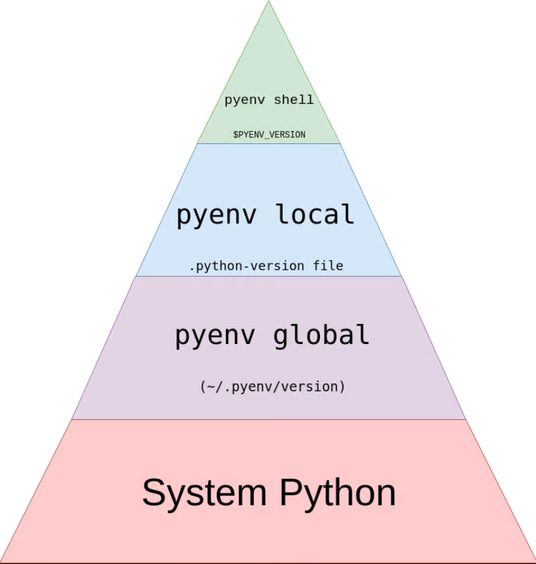
\includegraphics[width=0.5\textwidth]{IMG/pyenv.png} 
    \caption{Ordre de résolution des commandes \textbf{pyenv}}
\end{figure}

Voyons un exemple rapide :
\begin{lstlisting}[style=bash]
|\userprompt| pyenv versions
* system (set by /home/utilisateur/.pyenv/version)
  3.12.10
  3.14.0a7
\end{lstlisting}

Ici, c'est le système Python qui est utilisé.
\begin{lstlisting}[style=bash]
|\userprompt| pyenv global 3.14.0a7
|\userprompt| pyenv versions
  system
  3.12.10
* 3.14.0a7 (set by /home/utilisateur/.pyenv/version)
\end{lstlisting}

\textbf{pyenv} utilise maintenant \textbf{3.14.0a7} comme version de \textbf{Python}. Il indique même l'emplacement du fichier qu'il a trouvé. Ce fichier existe effectivement :
\begin{lstlisting}[style=bash]
|\userprompt| cat ~/.pyenv/version
3.14.0a7
\end{lstlisting}

Maintenant, créons un fichier \textbf{.python-version} avec \texttt{local} :
\begin{lstlisting}[style=bash]
|\userprompt| pyenv local 3.12.10
|\userprompt| pyenv versions
  system
* 3.12.10 (set by /home/utilisateur/.python-version)
  3.14.0a7
|\userprompt| cat .python-version
3.12.10
\end{lstlisting}

\textbf{pyenv} indique comment il doit résoudre la commande python. Cette fois, elle provient de \textbf{~/.python-version}. A Noter que la recherche de \textbf{.python-version} est récursive.
\begin{lstlisting}[style=bash]
|\userprompt| pyenv shell 3.14.0a7
|\userprompt| pyenv versions
  system
  3.12.10
* 3.14.0a7 (set by PYENV_VERSION environment variable)
\end{lstlisting}

Tout ce que cela a fait, c'est définir la variable d'environnement \texttt{\$PYENV\_VERSION} :
\begin{lstlisting}[style=bash]
|\userprompt| echo $PYENV_VERSION
3.14.0a7
\end{lstlisting}

\section{Environnement virtuel et \textit{pyenv}}
\textbf{pyenv} allié à un environnement virtuel est un mariage parfait. \textbf{pyenv} dispose d'un \textit{plugin} appelé \textbf{pyenv-virtualenv} qui permet de travailler avec plusieurs versions de Python et plusieurs environnements virtuels en un clin d'œil.
\begin{description}
    \item[pyenv] gère plusieurs versions de Python.
    \item[virtualenv/venv] gère les environnements virtuels pour une version spécifique de Python.
    \item[pyenv-virtualenv] gère les environnements virtuels pour différentes versions de Python.
\end{description}

\subsection*{Création d'un environnement virtuel}
\begin{lstlisting}[style=bash]
|\userprompt| pyenv virtualenv <version_python> <nom_environnement>
\end{lstlisting}

Une bonne pratique consiste à nommer les environnements du même nom que le projet. Par exemple, en travaillant sur \texttt{mon\_projet} développé avec \textbf{Python 3.6.8} :
\begin{lstlisting}[style=bash]
|\userprompt| pyenv virtualenv 3.6.8 mon_projet
\end{lstlisting}

\subsection*{Activation}
\begin{lstlisting}[style=bash]
|\userprompt| pyenv local mon_projet
\end{lstlisting}

Cela crée un fichier \textbf{.python-version} dans le répertoire de travail actuel et l'environnement sera automatiquement activé.

Vérification :
\begin{lstlisting}[style=bash]
|\userprompt| pyenv which python
/home/utilisateur/.pyenv/versions/my_project/bin/python
\end{lstlisting}

Une nouvelle version a été créée sous le nom de \texttt{my\_project} et l'exécutable python pointe vers cette version. En regardant n'importe quel exécutable fourni par cet environnement, nous verrons la même chose. Prenons, par exemple, \textbf{pip} :
\begin{lstlisting}[style=bash]
|\userprompt| pyenv which pip
/home/utilisateur/.pyenv/versions/my_project/bin/pip
\end{lstlisting}

Activer / Désactiver :
\begin{lstlisting}[style=bash]
|\userprompt| pyenv activate <nom_environnement>
|\userprompt| pyenv deactivate
\end{lstlisting}

\section{Travailler avec plusieurs environnements}
Supposons ces diverses versions de Python installées :
\begin{lstlisting}[style=bash]
|\userprompt| pyenv versions
* system (set by /home/user/.pyenv/version)
  3.11.12
  3.14.0a7
\end{lstlisting}

Par défaut, c'est le système Python qui est utilisé.

Nous souhaitons maintenant travailler sur deux projets différents :
\begin{itemize}
    \item \textbf{projet\_1}, qui supporte \textbf{Python 3.11.12}.
    \item \textbf{projet\_2}, qui supporte \textbf{Python 3.14.0a7}.
\end{itemize}

Créons un environnement virtuel pour chaque projet :
\begin{lstlisting}[style=bash]
|\userprompt| mkdir projet_1 projet_2
|\userprompt| cd projet_1
|\userprompt| pyenv which python3
/usr/bin/python3
|\userprompt| pyenv virtualenv 3.11.12 projet_01
|\userprompt| pyenv local projet_01
|\userprompt| python3 -V
Python 3.11.12
|\userprompt| cd ../projet_2
|\userprompt| pyenv which python3  # En changeant de répertoire on revient au système Python
/usr/bin/python3
|\userprompt| pyenv virtualenv 3.14.0a7 projet_02
|\userprompt| pyenv local projet_02
|\userprompt| python3 -V
Python 3.14.0a7
\end{lstlisting}

Plus besoin de se rappeler d'activer les environnements : en passant d'un projet à l'autre, \textbf{pyenv} se charge d'activer automatiquement les bonnes versions de Python et les bons environnements virtuels
\bigskip

\begin{center}
    \pgfornament[width=0.3\textwidth]{88} % 88 est le numéro de l'ornement
\end{center}

\textbf{pyenv} est donc un outil puissant qui permet de gérer efficacement différentes versions de Python. Grâce à lui nous pouvons désormais basculer entre les versions de Python avec une facilité déconcertante, optimisant ainsi nos environnements de développement pour répondre aux besoins spécifiques de chaque projet. Cependant, la gestion des dépendances et des paquets reste un aspect crucial du développement Python. Dans le chapitre suivant, nous allons nous plonger dans les potentialités de \textbf{poetry}, un outil moderne qui simplifie la gestion des dépendances et des environnements virtuels, nous permettant de gérer nos projets Python avec une grande précision. 

